%--------------------------------------
% Create title frame
\titleframe

%--------------------------------------
% Table of contents
\begin{frame}{Overview}
  \setbeamertemplate{section in toc}[sections numbered]
  \tableofcontents[hideallsubsections]
\end{frame}



%--------------------------------------


\begin{frame} {Leçons précédentes}
	\begin{itemize}
	\item Circuits linéaires, résistances, sources (commandées ou non) de courant et de tension.
	\item Lois de Kirchhoff
	\item Régime transitoire, éléments L et C.
	\end{itemize}
	\vfill
\end{frame}

\begin{frame}[allowframebreaks]{Qu'allons nous faire dans ce cours ?}
	Nous étudions les mêmes circuits que précédemment, mais nous introduisons des sources de courants et de tension qui fournissent un signal sinusoïdal. 
	\vfill 
	En régime établi et lorsque les éléments du systèmes sont linéaires et invariants, nous montrons qu'il est possible de simplifier l'analyse du système par l'introduction des phaseurs. 
	\vfill 	
	Moyennant la généralisation de la notion de résistance (resp. conductance) à la notion d'impédance (resp. admittance),  l'utilisation des phaseurs permet de continuer à employer les méthodes vues jusqu'à présent pour déterminer l'état électrique du système, en simplifier la représentation lorsqu'il est vu d'un nombre réduit d'accès, etc. Les phaseurs permettent également de grandement simplifier l'analyse des régimes transitoires via l'analyse fréquentielle.
	\vfill 
	Notions mathématiques utilisées : les mêmes que précédemment, mais les nombres complexes sont maintenant omniprésents.
	\vfill 
	\textbf{Dans le syllabus : }
\begin{itemize}
  \item Les sections 1 à 4 du chapitre 4
  \item Exercices 4.1 à 4.5, 4.8.1.
\end{itemize}
\end{frame}

%-------------------------------------------------------------------------------

\section{Source sinusoïdale et phaseur}
\subsection{Source sinusoïdale}
\begin{frame}{Qu'est-ce qu'une source sinusoïdale ? }
	
	C'est une source indépendante qui délivre une tension (ou un courant) de forme
	sinusoïdale (ou cosinusoïdale, un sin = cos déphasé).
	\vfill
	\begin{columns}
		\begin{column}{0.7\linewidth}
		\centering
		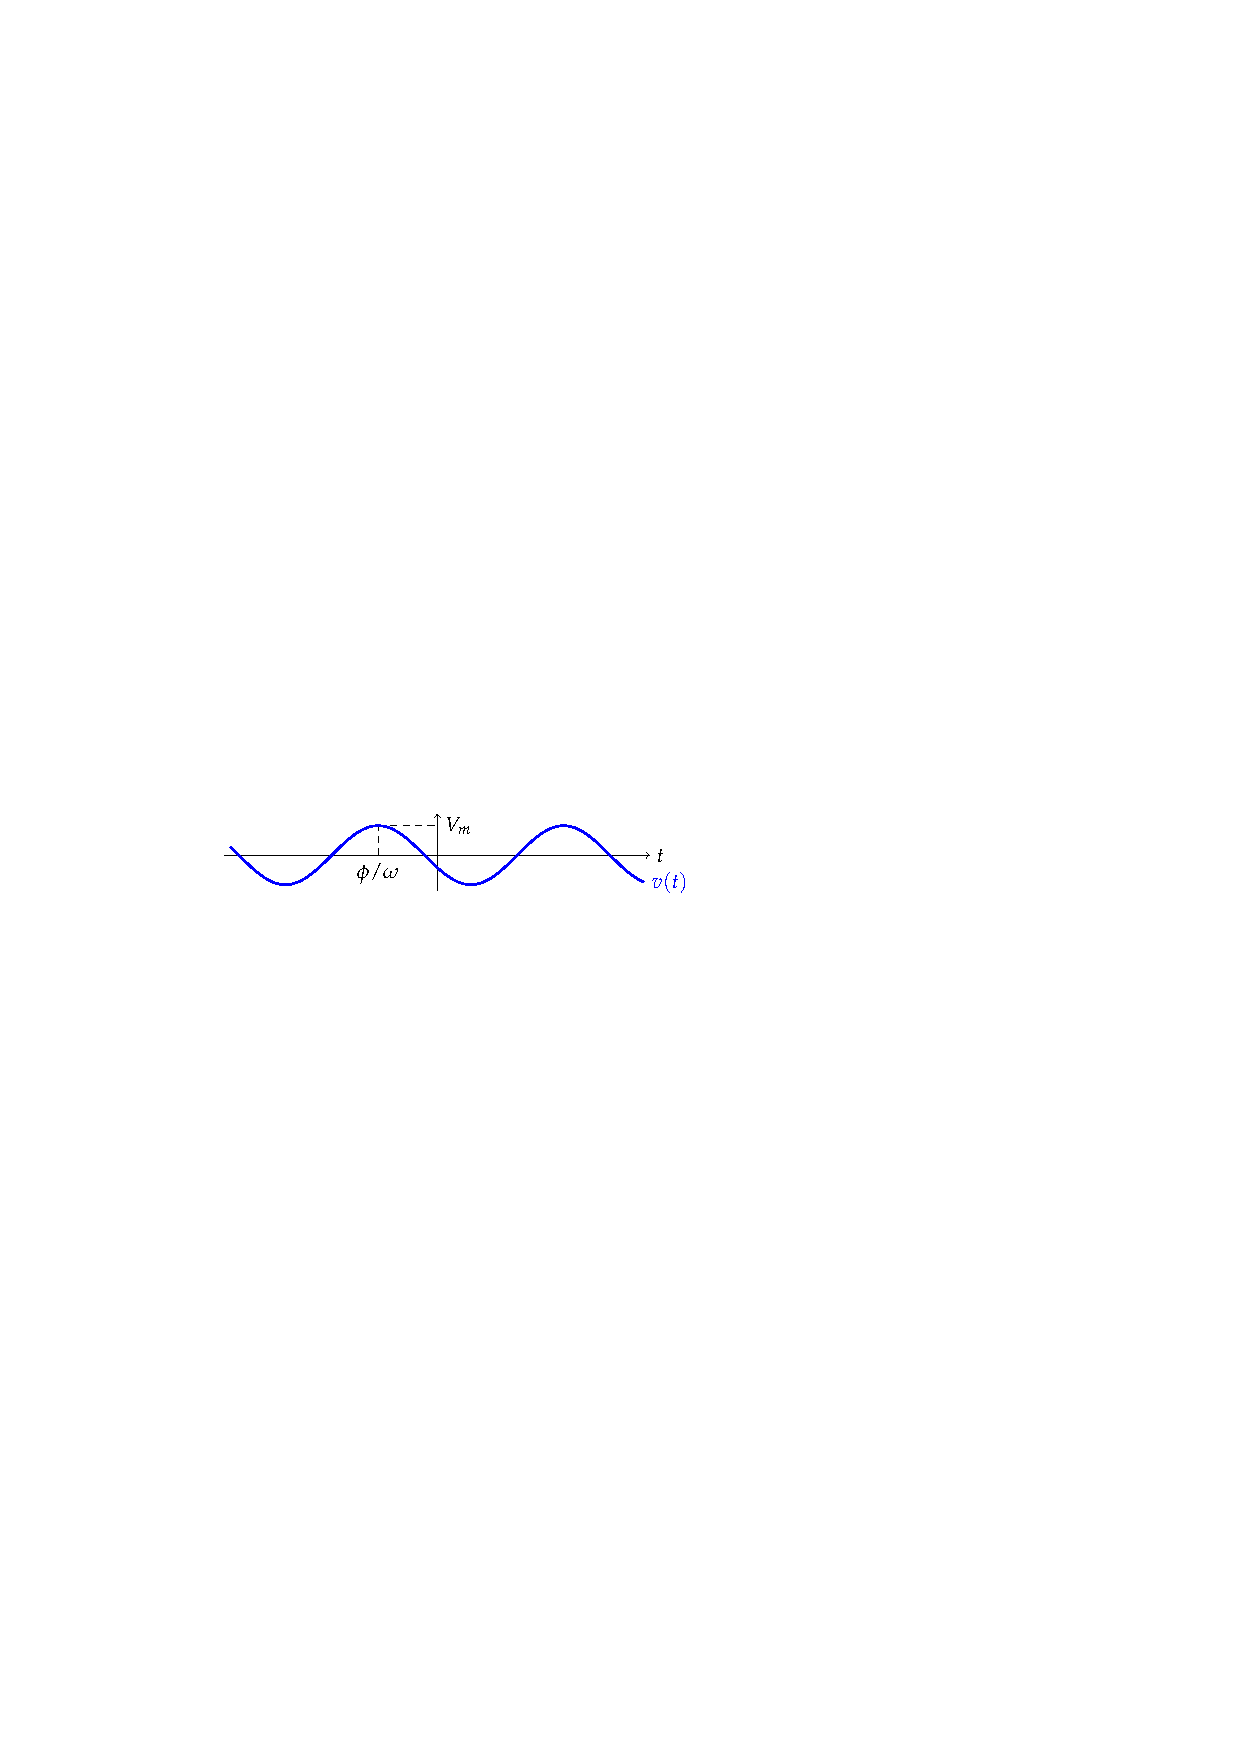
\includegraphics[width=0.7\linewidth]{figs/source_sin}
		\end{column}
		\begin{column}{0.25\linewidth}
		\[v(t)=V_m\cos(\omega t +\phi)\]
		\end{column}
	\end{columns}
	\vfill
	Signal périodique : 
	\begin{itemize}
		\item période : $T=\frac{2\pi}{\omega}$ s
		\item fréquence : $f=\frac{1}{T}=\frac{\omega}{2\pi}$ Hz
		\item pulsation : $\omega$ rad/s
		\item phase : $\phi$ rad
	\end{itemize}
	
	On désigne aussi parfois ce signal par ``signal cissoïdal''\\
\end{frame}

%-------------------------------------------------------------------------------

\begin{frame}{Un signal sinusoïdal est donc entièrement déterminé par}
	\begin{itemize}
		\item son {\bf  amplitude} sous forme de la valeur maximale $V_m$ (aussi dénommée valeur de crête) 
		\item sa \textbf{fréquence} $f$
		\item sa \textbf{phase} $\phi$
	\end{itemize}
\end{frame}


\begin{frame}{Pourquoi des sources sinusoïdales ?}

  \begin{itemize}
    \item Le transport et la distribution d'électricité fonctionnent majoritairement en courant alternatif (50 Hz en Europe) : 
    \begin{itemize}
      \item les machines tournantes des centrales tournent (à un multiple) de cette fréquence
      \item le courant alternatif permet l'utilisation de transformateurs (cf. prochaine leçon) pour élever les niveaux de tension et diminuer les pertes
    \end{itemize} 
    \item Les signaux complexes peuvent êtres vus comme une \textbf{superposition} de signaux sinusoïdaux à différentes fréquences, phases et amplitudes (c.f. analyse de Fourier)
  \end{itemize}

\end{frame}

\begin{frame}{Valeur efficace}
Plutôt que par sa valeur de crête, on caractérise souvent un signal par sa \textbf{valeur efficace}.
\begin{block}{Valeur efficace}
\begin{eqnarray*}
	V_{\text {eff}}& =&\sqrt{\frac{1}{T}\int_{t_0}^{t_0+T}V_m^2\cos^2(\omega t + \phi)dt}\\
	& = & \frac{V_m}{\sqrt{2}} \simeq 0.707 V_m
\end{eqnarray*}
\end{block}
\vfill
C'est la valeur que devrait présenter une tension continue pour dissiper dans
une résistance une puissance égale à la puissance {\em moyenne}
dissipée par la tension sinusoïdale.
\vfill 

Par la suite, on désignera $V_{\text{eff}}$ par $V$ !!
\end{frame}
%-------------------------------------------------------------------------------

\subsection{Notion de phaseur}
\begin{frame}{Notion de phaseur}

  \begin{columns}
    \begin{column}{0.65\textwidth}
      \textbf{Un phaseur est un nombre complexe associé à une grandeur  sinusoïdale} $A_m\cos(\omega t+\phi)=\sqrt{2}A\cos(\omega t+\phi)$:
      \[\bar{A}= A e^{j\phi}=A\angle \phi\]
      
      On \textbf{associe aussi à un phaseur un vecteur tournant} $e^{j\omega t}$ :
      \[\bar{A} e^{j\omega t}\]
      Il peut être représenté dans le plan complexe par un vecteur tournant
      à la vitesse angulaire $\omega$. Le phaseur correspond à la position de
      ce vecteur en $t=0$. 
  \end{column}
  \begin{column}{0.3\textwidth}
    \begin{center}
    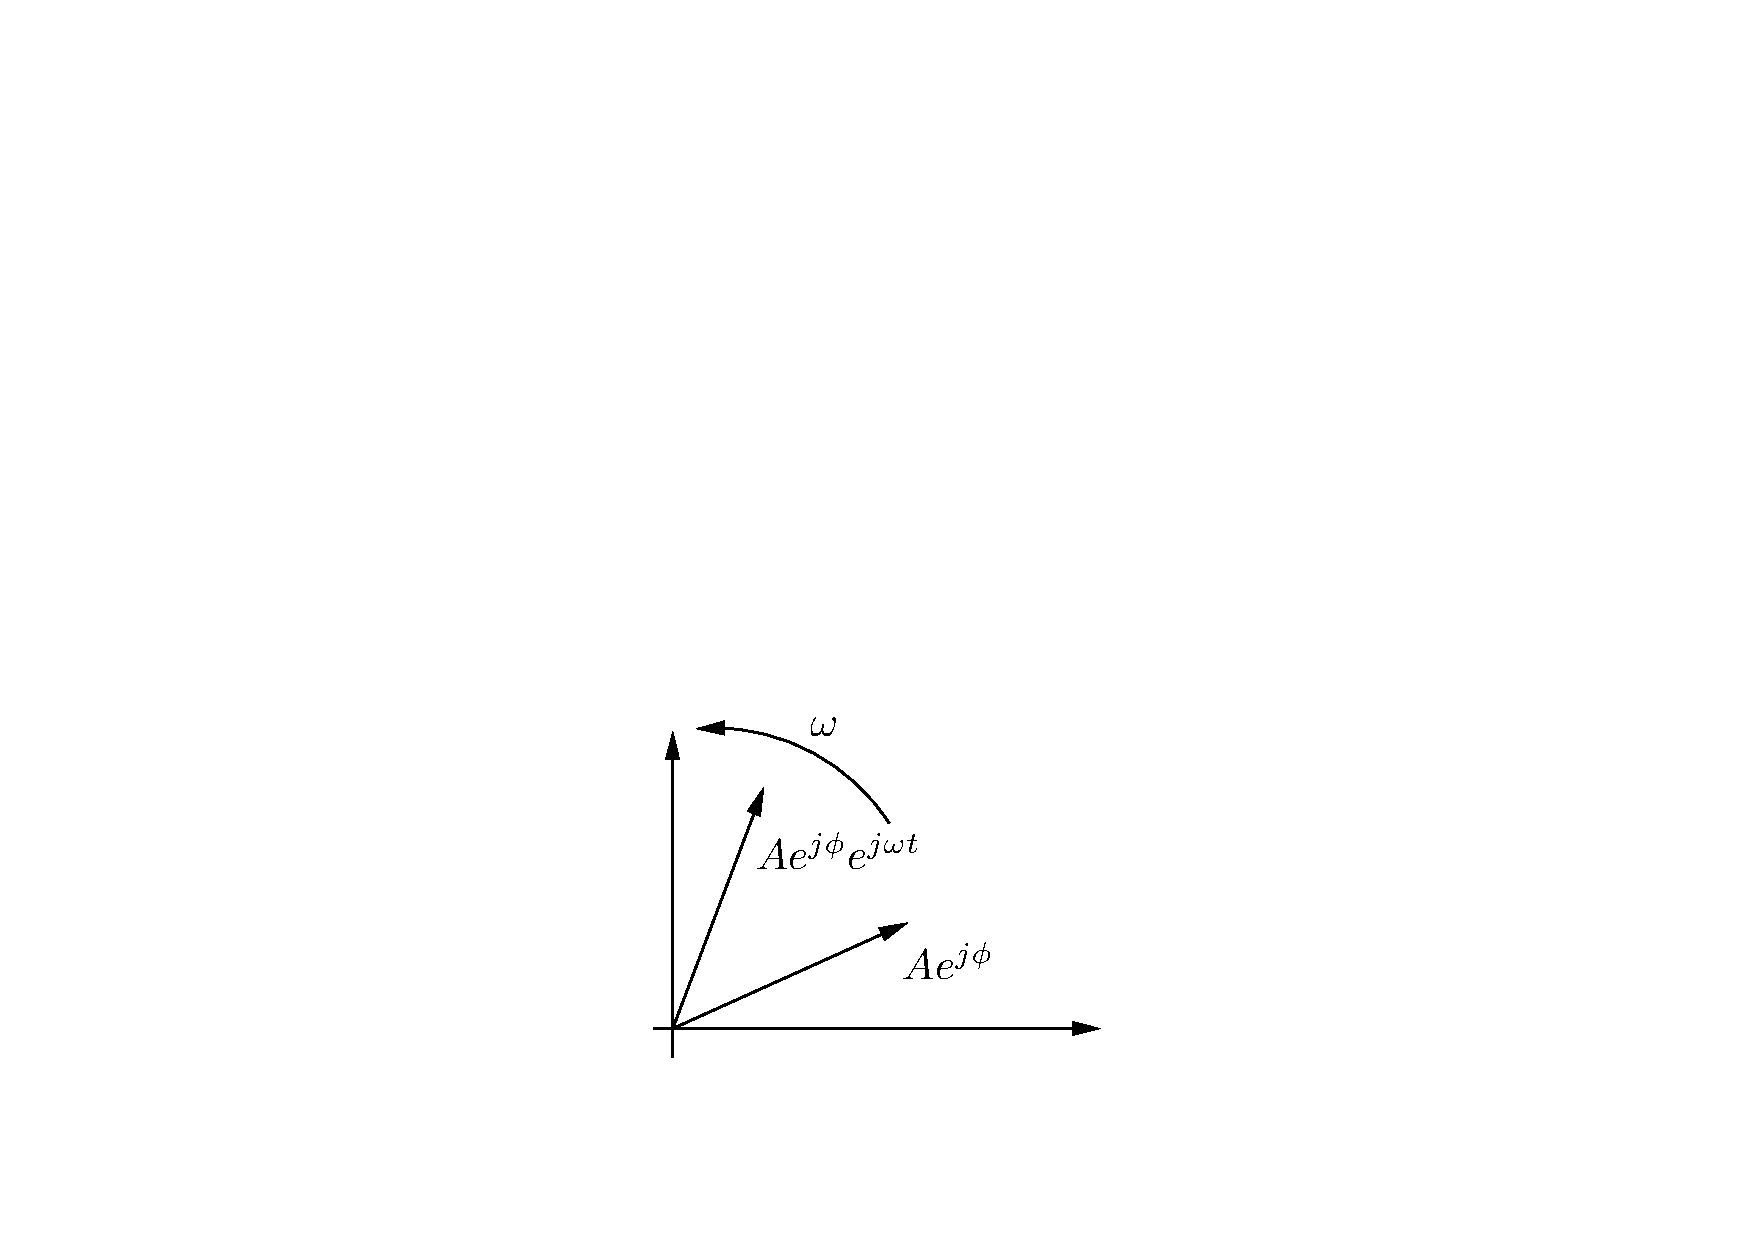
\includegraphics[width=\linewidth]{figs/phaseur_def}
    \end{center}
  \end{column}
  \end{columns}
	
\end{frame}

%-------------------------------------------------------------------------------

\begin{frame}{\Large Correspondance biunivoque entre signal sinusoïdal et phaseur}
	\[
	\begin{array}{rcl}
	\text{Sinusoïde} & & \text{Phaseur}\\
	\left.\begin{array}{r}
	A_m\cos(\omega t+\phi)\\
	=(A_m\cos \phi)\cos \omega t \\
	+(-A_m\sin \phi)\sin \omega t
	\end{array}\right\} &
	\Leftrightarrow & 
	\left\{\begin{array}{l}
	\bar{A}=A e^{j\phi}\\
	= (A \cos \phi)\\
	+j(A \sin \phi)
	\end{array}\right.
	\end{array}\]
	\begin{eqnarray*}
		A_m\cos(\omega t + \phi) & = &\text{Re}[\sqrt{2} \bar A e^{j\omega t}]\\
		& = & \text{Re}[\sqrt{2}\bar A]\cos \omega t - \text{Im}[\sqrt{2}\bar A]\sin \omega t
	\end{eqnarray*}


\textbf{Un phaseur contient donc deux des trois éléments qui caractérisent un signal sinusoidal : son amplitude et sa phase. }

La troisième est souvent implicite. Par exemple, on sait si on est en Europe et qu'on s'intéresse au réseau électrique que la fréquence du réseau vaut 50 Hz.
	
%	On peut aussi définir le phaseur à partir de la valeur maximale du signal :
%	\[\bar{A}=A_m e^{j\phi}\]
	
\end{frame}

%-------------------------------------------------------------------------------

\subsection{Propriétés des phaseurs}
\begin{frame}[allowframebreaks]{Propriétés des phaseurs -- linéarité}
	
	\begin{block}{Linéarité}
	Le phaseur correspondant à une combinaison linéaire de signaux sinusoïdaux est égal à la combinaison linéaire des phaseurs des différents signaux.
	\end{block}
	
	Soient deux signaux sinusoïdaux :
	\[v_1(t)=\text{Re}[\sqrt{2}\bar{V}_1e^{j\omega t}] \quad \text{et}
	\quad v_2(t)=\text{Re}[\sqrt{2}\bar{V}_2e^{j\omega t}]\]
	
	Une combinaison linéaire :
	\[a_1v_1(t)+a_2v_2(t)=
	a_1\text{Re}[\sqrt{2}\bar{V}_1e^{j\omega t}] +
	a_2\text{Re}[\sqrt{2}\bar{V}_2e^{j\omega t}]\]
	
	avec $a_1$ et $a_2$, 2 nombres réels.
	
	\[a_1\text{Re}[\sqrt{2}\bar{V}_1e^{j\omega t}] +
	a_2\text{Re}[\sqrt{2}\bar{V}_2e^{j\omega t}] =
	\text{Re}[\sqrt{2}(a_1\bar{V}_1+a_2\bar{V}_2)e^{j\omega t}]\]
	
	La combinaison linéaire des signaux est représentée par le phaseur :
	\[a_1\bar{V}_1+a_2\bar{V}_2\]
\end{frame}

%-------------------------------------------------------------------------------

\begin{frame}{Propriétés des phaseurs -- dérivation}
	
	\begin{block}{Dérivation}
	\[\frac{d}{dt}\left(V_m\cos(\omega t+\phi)\right)\,\,\Leftrightarrow\,\,
	j\omega \bar{V}\]
	\end{block}
	
	\begin{eqnarray*}
		\frac{d}{dt}\left(V_m\cos(\omega t+\phi)\right)& = &
		-\omega V_m\sin(\omega t+\phi) \\
		& = &\text{Re}[j\omega V_me^{j(\omega t + \phi)}]\\
		& = &\text{Re}[j\omega V_me^{j\phi}e^{j\omega t}]= \text{Re}[j\omega \sqrt{2}\bar{V}e^{j\omega t}]
	\end{eqnarray*}
	\begin{center}
		\fbox{
			$\frac{d}{dt}\left(\text{Re}[\bar{V}e^{j\omega t}]\right)= 
			\text{Re}[\frac{d}{dt}\left( \bar{V}e^{j\omega t}\right)]=
			\text{Re}[j\omega \bar{V}e^{j\omega t}]$}
	\end{center}
	
\end{frame}

%-------------------------------------------------------------------------------

\begin{frame}{Propriétés des phaseurs -- intégration}
	
	\begin{block}{Intégration}
	\[\int V_m\cos(\omega t+\phi)\ dt\,\,\Leftrightarrow\,\,
	\frac{\bar{V}}{j\omega}\]
	\end{block}
	
	\begin{equation}
		\int V_m\cos(\omega t+\phi)\, dt = 
		\frac{V_m}{\omega}\sin(\omega t+\phi) = \text{Re}[\frac{V_me^{j\phi}e^{j\omega t}}{j \omega}] = \text{Re}[\frac{\sqrt{2}\bar{V}}{j \omega}e^{j\omega t}]
	\end{equation}
	\begin{center}
		\fbox{$\int \text{Re}[\bar{V}e^{j\omega t}]\, dt =
			\text{Re}[\int \bar{V}e^{j\omega t}\, dt]=
			\text{Re}[\frac{\bar{V}}{j\omega} e^{j\omega t}]$}
	\end{center}
\end{frame}

%-------------------------------------------------------------------------------

\section{Réponse à une excitation sinusoïdale}
\begin{frame}{Exemple : circuit RL}
	
	\begin{columns}
		\begin{column}{0.6\linewidth}	
		\begin{center}
		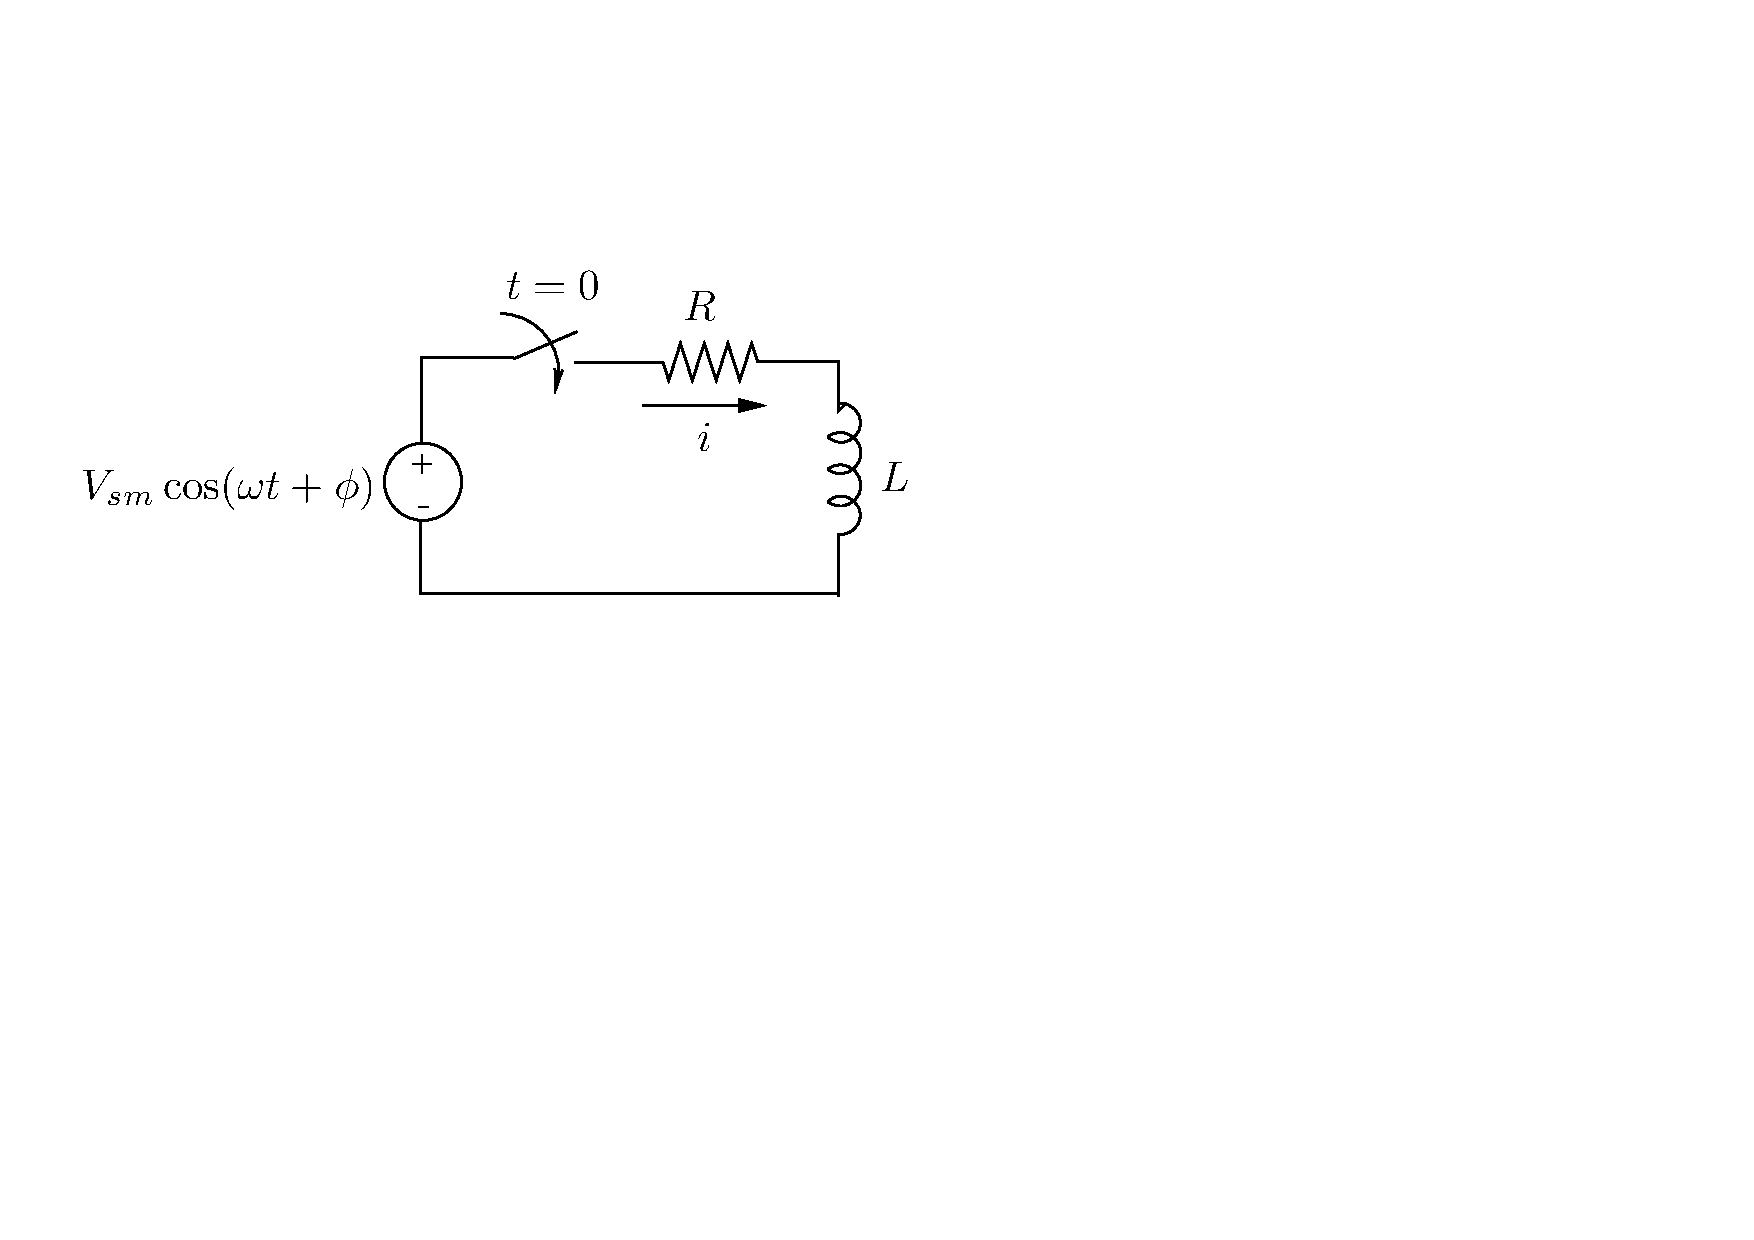
\includegraphics[width=0.7\linewidth]{figs/reponse_sin}
		\end{center}
		\end{column}
		\begin{column}{0.4\linewidth}
			$L$ initialement relaxée
			
			Courant $i(t)$ solution de 
			\[L\frac{di}{dt}+R\, i=V_{sm}\cos(\omega t+\phi)\]
		\end{column}
	\end{columns}
	\vfill 
	Solution de la forme :
	\[K_1e^{-t/\tau} + I_m\cos(\omega t+\theta)\]
	
	\begin{itemize}
		\item $K_1e^{-t/\tau}$ : solution de l'équation homogène : représente la réponse transitoire 
		\item $I_m\cos(\omega t+\theta)$ \alert{solution particulière} \\
		représente la réponse permanente = réponse en \alert{régime sinusoïdal établi}
	\end{itemize} 
\end{frame}

%-------------------------------------------------------------------------------

\begin{frame}{\large Recherche de la solution en régime sinusoïdal établi à partir des
		phaseurs}
	
	Soit $i(t)=I_m\cos(\omega t+\theta)=\text{Re}[\sqrt{2}\bar{I}e^{j\omega t}]$
	avec le phaseur $\bar{I}=I e^{j\theta}$
	\begin{gather*}
	L\frac{d}{dt}\left(\text{Re}[\sqrt{2}\bar{I}e^{j\omega t}]\right)+R\, \text{Re}
	[\sqrt{2}\bar{I}e^{j\omega t}]= \text{Re}[\sqrt{2}\bar{V}_se^{j\omega t}]\\
	\text{Re}[j\omega L \sqrt{2}\bar{I}e^{j\omega t}]+ \, \text{Re}
	[R\sqrt{2} \bar{I}e^{j\omega t}]= \text{Re}[\sqrt{2}\bar{V}_se^{j\omega t}]\\
	\text{Re}[(j\omega L+R)  \bar{I}e^{j\omega t}]= \text{Re}[\bar{V}_se^{j\omega t}]
	\end{gather*}
	Equation \alert{algébrique} pour les phaseurs :
	\begin{gather*}
	(j\omega L+R)  \bar{I}=\bar{V}_s \quad \rightarrow \quad \bar{I} =
	\frac{\bar{V}_s}{j\omega L+R}=I e^{j\theta}\\
	I =\frac{V_{s}}{\sqrt{\omega^2 L^2+ R^2}}, \quad \theta = \phi -
	\arctan \frac{\omega L}{R}
	\end{gather*}
\end{frame}

%-------------------------------------------------------------------------------

\section{Lois de la théorie des circuits et phaseurs}
\begin{frame}{Lois de la théorie des circuits et phaseurs}
	
	Toutes les relations linéaires du domaine temporel se transforment en
	relations algébriques équivalentes entre les phaseurs du domaine
	fréquentiel.
	\vfill
	
	\begin{block}{Attention :}
		\begin{itemize}
			\item Cette propriété ne s'applique qu'aux
			relations linéaires; \\contre-exemple : calcul des puissances. 
			\item Tous les éléments constituant le circuit doivent être linéaires et
			invariants.
		\end{itemize}
	\end{block}
	\end{frame}
	
	%-------------------------------------------------------------------------------
	
	\subsection{Lois de Kirchhoff}
	\begin{frame}{Lois de Kirchhoff}
		
		PLK : 
		\[ \boxed{i_1(t)+i_2(t)+\ldots i_k(t) =0 \quad \Leftrightarrow \quad
		\bar{I}_1+ \bar{I}_2+\ldots \bar{I}_k=0}\]
		%(Sous forme matricielle :
		%\[{\bf A}\mathcolor{red}{\bar{\bf I}_B}={\bf 0}\]
		%avec ${\bf A}$ la matrice d'incidence aux noeuds (cf. dernier chapitre).)
		%\vfill 
		SLK :
		\[ \boxed{u_1(t)+u_2(t)+\ldots u_k(t) =0 \quad \Leftrightarrow \quad
		\bar{U}_1+ \bar{U}_2+\ldots \bar{U}_k=0}\]
		%(Sous forme matricielle :
		%\[{\bf B}\mathcolor{red}{\bar{\bf U}_B}={\bf 0}\]
		%avec ${\bf B}$ la matrice des mailles (cf. dernier chapitre).)
	\end{frame}
	
	%-------------------------------------------------------------------------------
	\subsection{Relations entre $u$ et $i$ de branches}
	\begin{frame}{Relations entre $u$ et $i$ de branches -- Résistance}
		
		\[u(t)=Ri(t) \quad \Leftrightarrow \bar{U}=R\, \bar{I}\]
		\[i(t)=I_m\cos(\omega t+\phi),\qquad u(t)=R\,I_m\cos(\omega t+ \phi)\]
		
		$u$ et $i$ sont en phase
		\begin{center}
			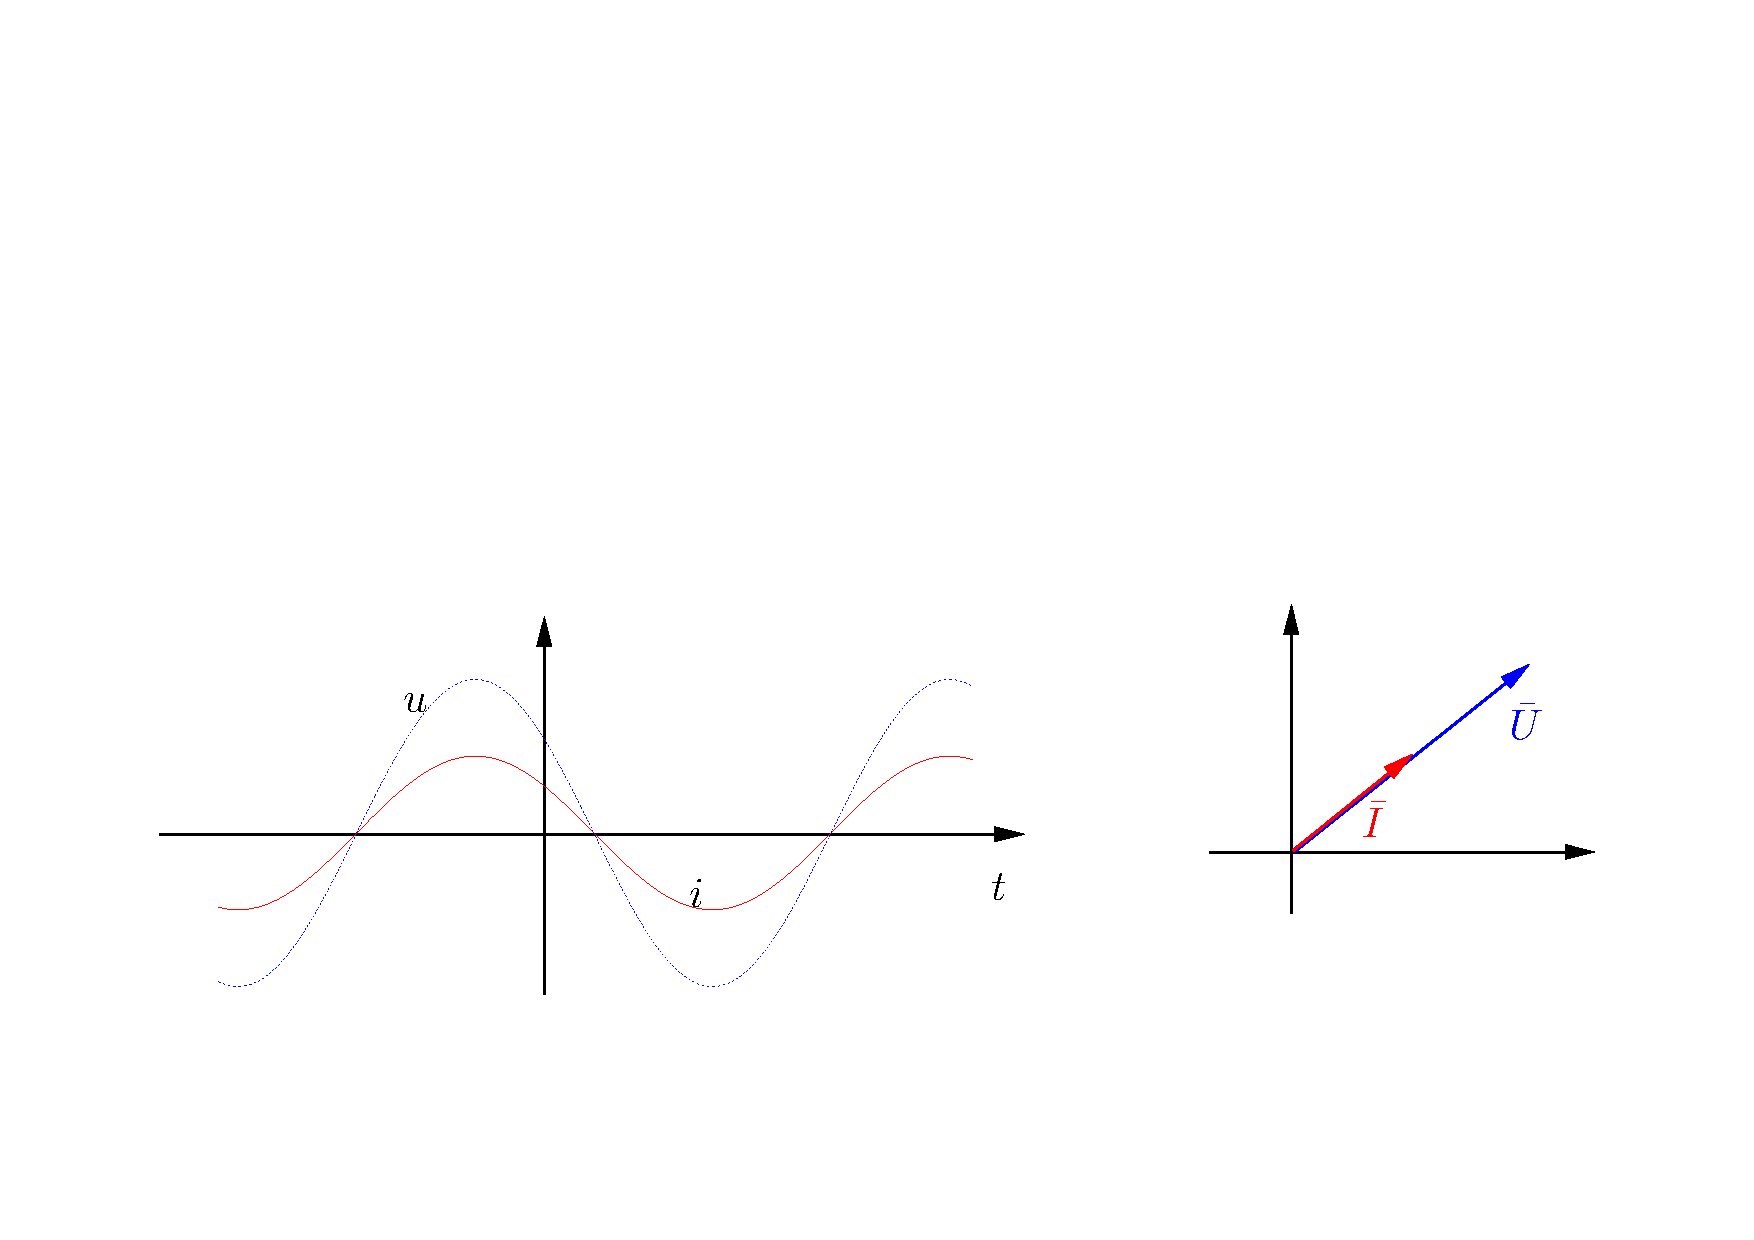
\includegraphics[width=0.9\linewidth]{figs/u_et_i_en_phase}
		\end{center}
	\end{frame}
	
	%-------------------------------------------------------------------------------
	
	\begin{frame}{Relations entre $u$ et $i$ de branches -- Inductance}
		{\small \[u(t)=L\frac{di(t)}{dt} \quad \Leftrightarrow \bar{U}=j\omega L\,
			\bar{I}\]
			\[i(t)=I_m\cos(\omega t+\phi),\qquad u(t)=\omega L\,I_m\cos(\omega t+
			\phi+\frac{\pi}{2})=
			-\omega L\,I_m\sin(\omega t+
			\phi)\]}
		$i$ en \alert{retard} de phase de $90^{\circ}$ par rapport à $u$
		\begin{center}
			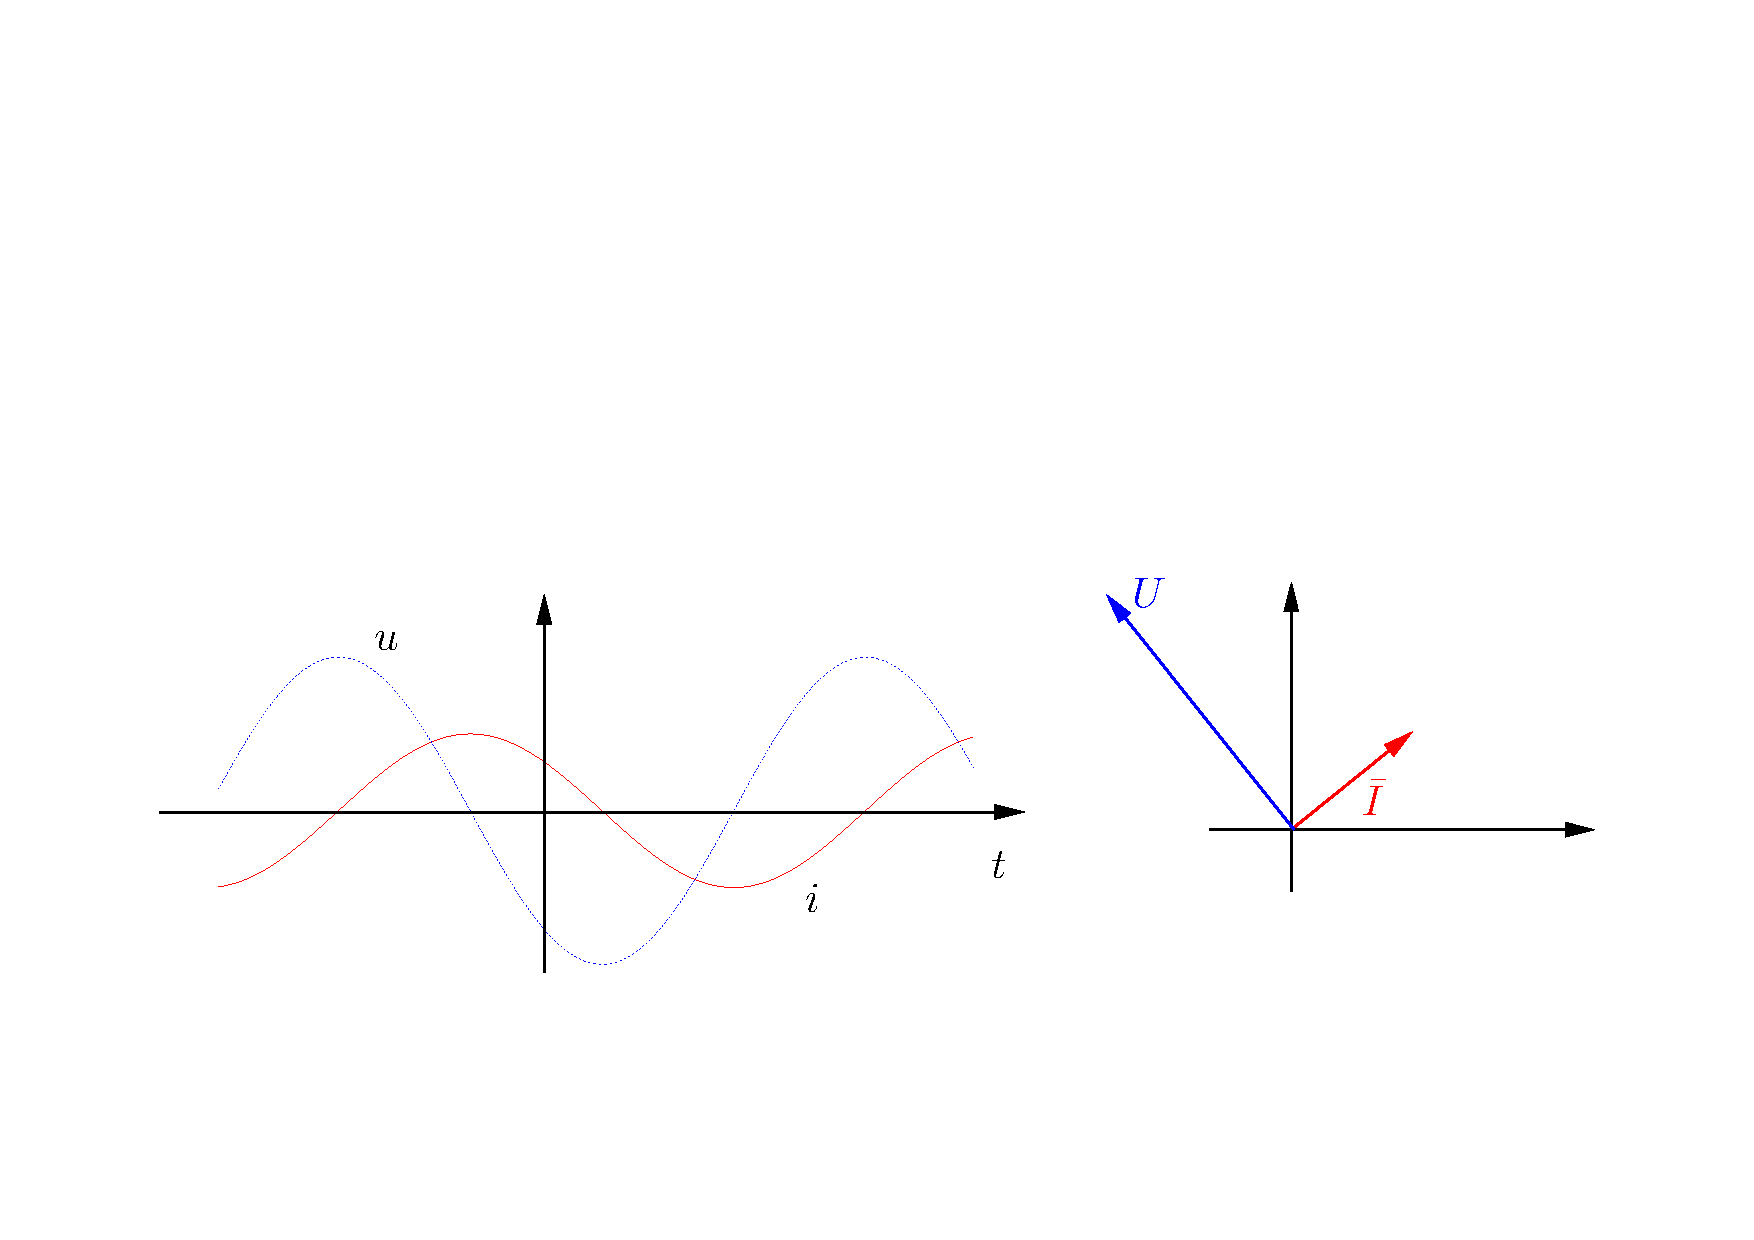
\includegraphics[width=0.8\linewidth]{figs/u_et_i_lag}
		\end{center}
	\end{frame}
	
	%-------------------------------------------------------------------------------
	
	\begin{frame}{Relations entre $u$ et $i$ de branches -- Condensateur}
		{\small \[u(t)=\frac{1}{C}\int i(x)dx \quad \Leftrightarrow \bar{U}=\frac{1}{j\omega C}
			\bar{I}\]
			\[i(t)=I_m\cos(\omega t+\phi),\qquad u(t)=\frac{I_m}{\omega C}\cos(\omega t+
			\phi-\frac{\pi}{2})=
			\frac{I_m}{\omega C}\sin(\omega t+
			\phi)\]}
      \vspace{-1cm}
		$i$ en \alert{avance} de phase de $90^{\circ}$ par rapport à $u$
		\begin{center}
			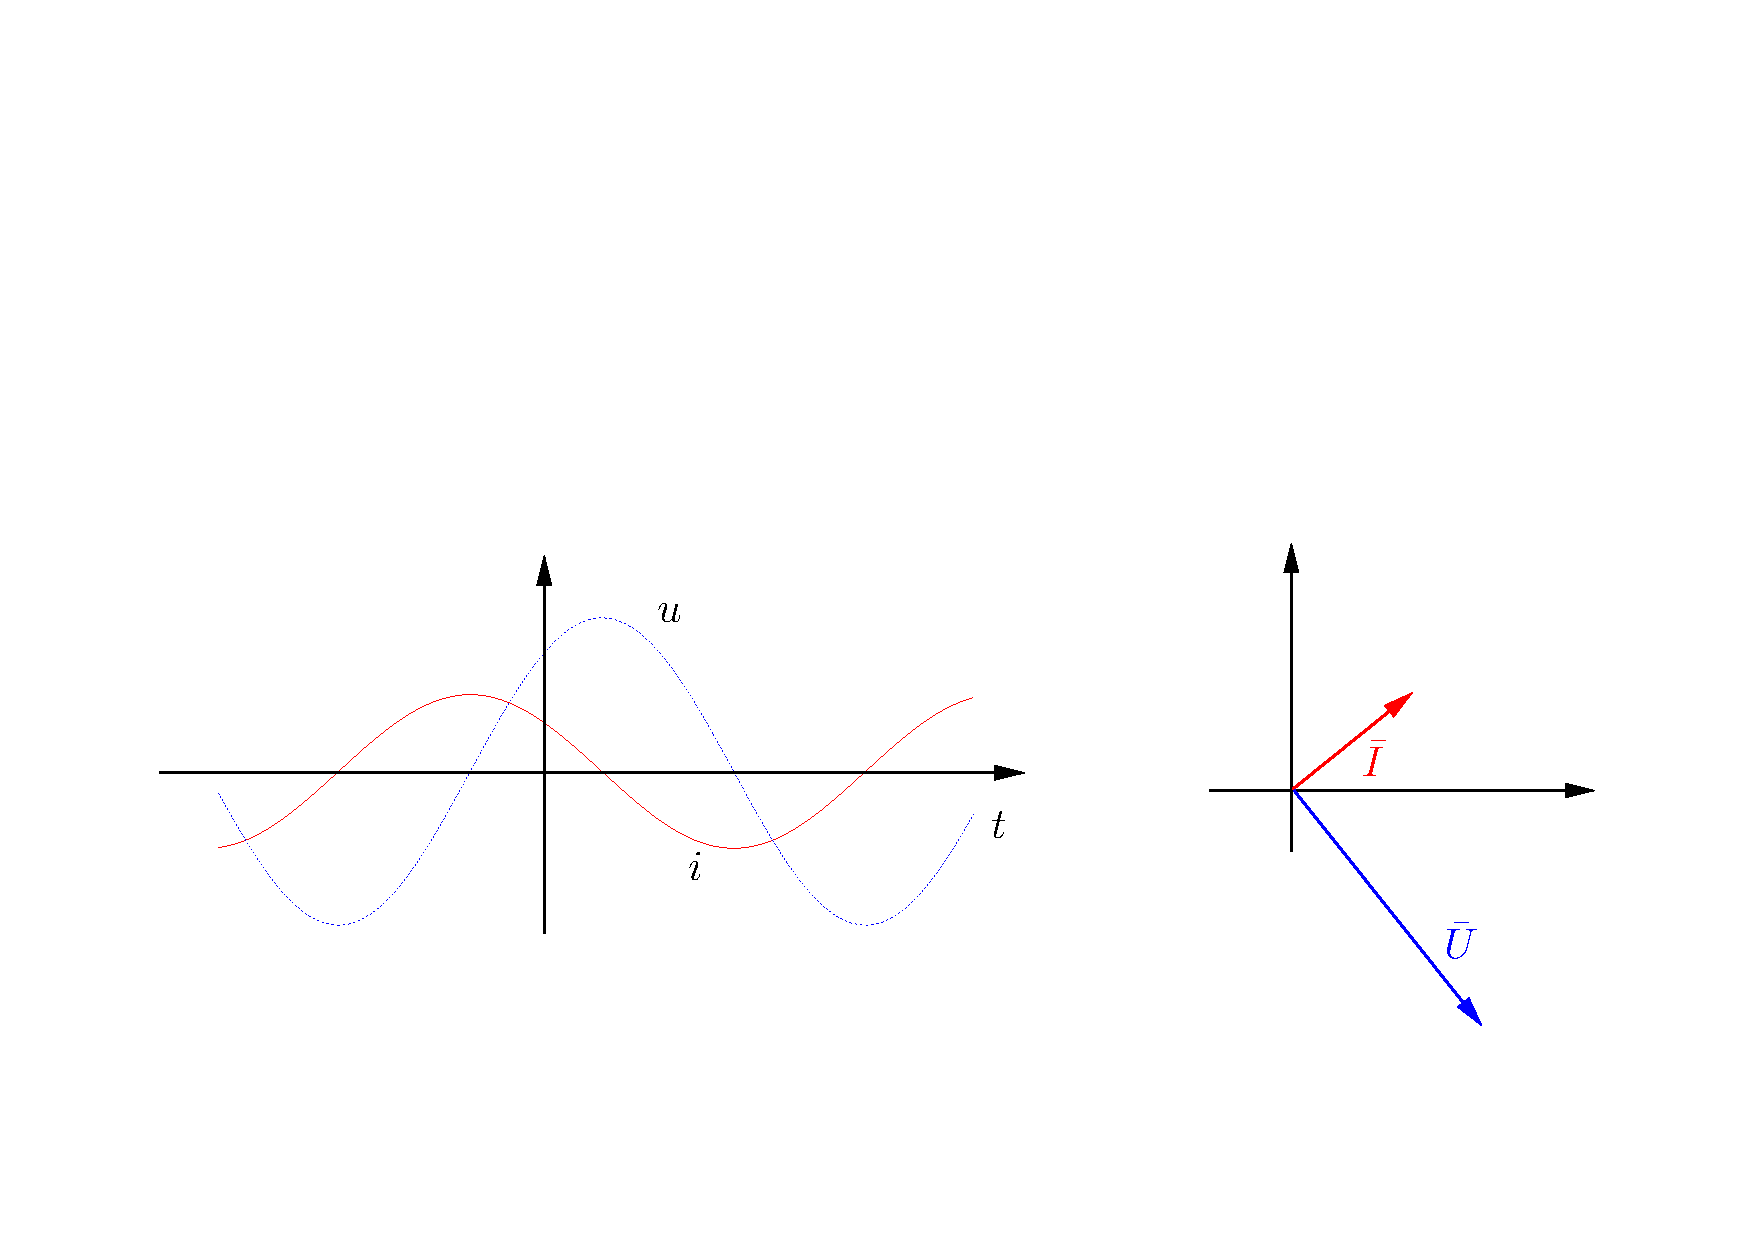
\includegraphics[width=0.8\linewidth]{figs/u_et_i_lead}
		\end{center}
	\end{frame}
	
	%-------------------------------------------------------------------------------
	
	\subsection{Notion d'impédance et d'admittance}
	\begin{frame}[allowframebreaks]{Notion d'impédance et d'admittance}
		
    \begin{columns}
    \begin{column}{0.55\textwidth}
      Soit $\cal R$ un dipôle \alert{passifié} comportant un certain nombre d'éléments
      linéaires et invariants interconnectés et fonctionnant en régime
      sinusoïdal établi. 
      
      \begin{itemize}
        \item $u(t)$ et $i(t)$ sont les tension et courant sinusoïdaux aux bornes de
        ce dipôle,\\
        \item $\bar{U}$ et $\bar{I}$ les phaseurs correspondants.
      \end{itemize}
    \end{column}
    \begin{column}{0.4\textwidth}
			\centering
			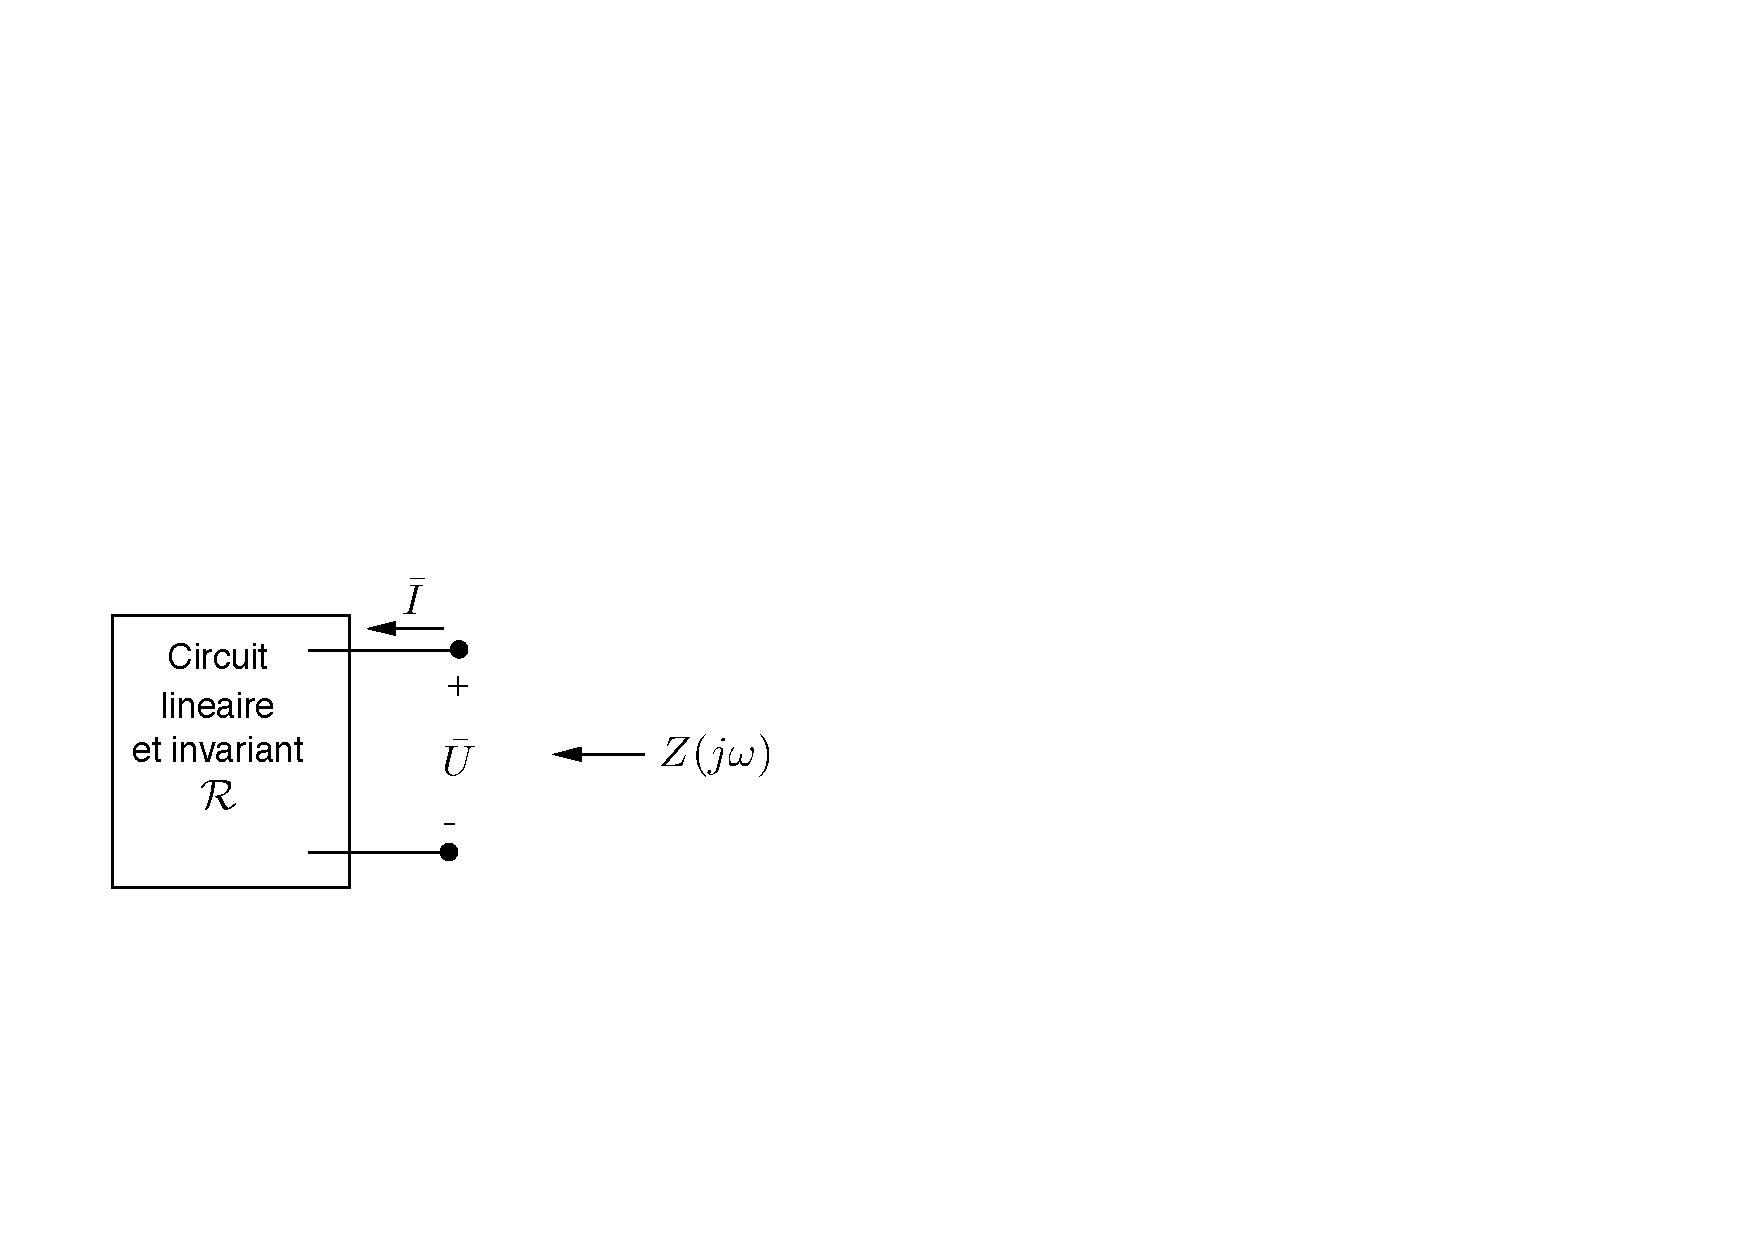
\includegraphics[width=\linewidth]{figs/circuit_equivalent}
    \end{column}
    \end{columns}
    \newpage
		\begin{columns}
			\begin{column}{0.47\linewidth}
			\begin{block}{Impédance}
					On appelle {\em impédance} du dipôle le rapport des phaseurs 
					\[Z(j\omega)=\frac{\bar{U}}{\bar{I}}\, ,\quad \bar{U}=Z\,\bar{I}\]
				\end{block}
			\end{column}
			\begin{column}{0.47\linewidth}
        \begin{block}{Admittance}
          L'inverse de l'impédance est l'{\em admittance}
          \[Y(j\omega)=\frac{\bar{I}}{\bar{U}}\, ,\quad \bar{I}=Y\,\bar{U}\]
        \end{block}
			\end{column}
		\end{columns}
\end{frame}

%-------------------------------------------------------------------------------

\begin{frame}[allowframebreaks]{\Large $Z =$ résistance $+ j$ réactance, $Y = $ conductance $+ j$ susceptance}
	
	$Z$ et $Y$ sont deux nombres complexes.
	
	\[Z=R+j\, X = |Z|e^{j\theta}\quad 
	\left\{
	\begin{array}{ll}
	R = \text{Re}[Z] = |Z|\cos \theta & \text{est la {\bf résistance}}\\
	X = \text{Im}[Z] = |Z|\sin \theta & \text{est la {\bf réactance}}\\
	|Z| = \sqrt{R^2+X^2} & \text{est le {\em module}}\\
	\theta = \arctan \frac{X}{R} & \text{est l'{\em argument}}
	\end{array}\right. \]
	
	
	\vspace*{2mm}
	\[Y=G+j\, B = |Y|e^{j\zeta} \quad
	\left\{\begin{array}{ll}
	G = \text{Re}[Y] = |Y|\cos \zeta & \text{est la {\bf conductance}}\\
	B = \text{Im}[Y] = |Y|\sin \zeta & \text{est la {\bf susceptance}}\\
	|Y| = \sqrt{G^2+B^2} & \text{est le {\em module}}\\
	\zeta = \arctan \frac{B}{G} & \text{est l'{\em argument}}\\
	\end{array}\right.\]
	\vfill
	\textbf{L'impédance et l'admittance ne sont pas des phaseurs !} Ils n'ont pas de vecteur tournant  ni de signal sinusoïdal associés.
\end{frame}

%-------------------------------------------------------------------------------

\begin{frame}{Impédance et admittance des composants de base}
	
	\begin{center}
		\begin{tabular}{l|ccc|ccc}
      \toprule
			Composant & Impéd. & Résist. & Réact. & Admitt. &
			Conduct. & Suscept. \\ 
      \midrule
			Résistance & $R$ & $R$ & -- & $\frac{1}{R}$ &   $\frac{1}{R}$ & --\\
			Inductance & $j\omega L$ & -- & $\omega L$ & $\frac{1}{j\omega L}$ &
			-- & $\frac{-1}{\omega L}$\\
			Condensateur & $\frac{1}{j\omega C}$ & -- & $\frac{-1}{\omega C}$ 
			& $j\omega C$ & -- &  $\omega C$ \\
      \bottomrule
		\end{tabular}
	\end{center}
\end{frame}


\begin{frame}{Associations en série et en parallèle}
\begin{itemize}
	\item Des \textbf{impédances} s'associent de la même manière que des \textbf{résistances}
	\item Des \textbf{admittances} s'associent de la même manière que des \textbf{conductances}	
\end{itemize}
\end{frame}

%-------------------------------------------------------------------------------

\begin{frame}{Exemple : impédance d'un circuit RLC série}
	
\begin{columns}
  \begin{column}{0.65\textwidth}
    \[Z(j\omega)=R+j\omega L+\frac{1}{j\omega C}\]
    \[|Z|=\sqrt{R^2 +(\omega L-\frac{1}{\omega C})^2}\, \quad
    \angle Z=\arctan \frac{ \omega L-\frac{1}{\omega C}}{R}\]
    \[\text{résistance :~}R \,, \quad \text{réactance :~}X= \omega
    L-\frac{1}{\omega C}\]
  \end{column}
  \begin{column}{0.3\textwidth}
    \begin{center}
      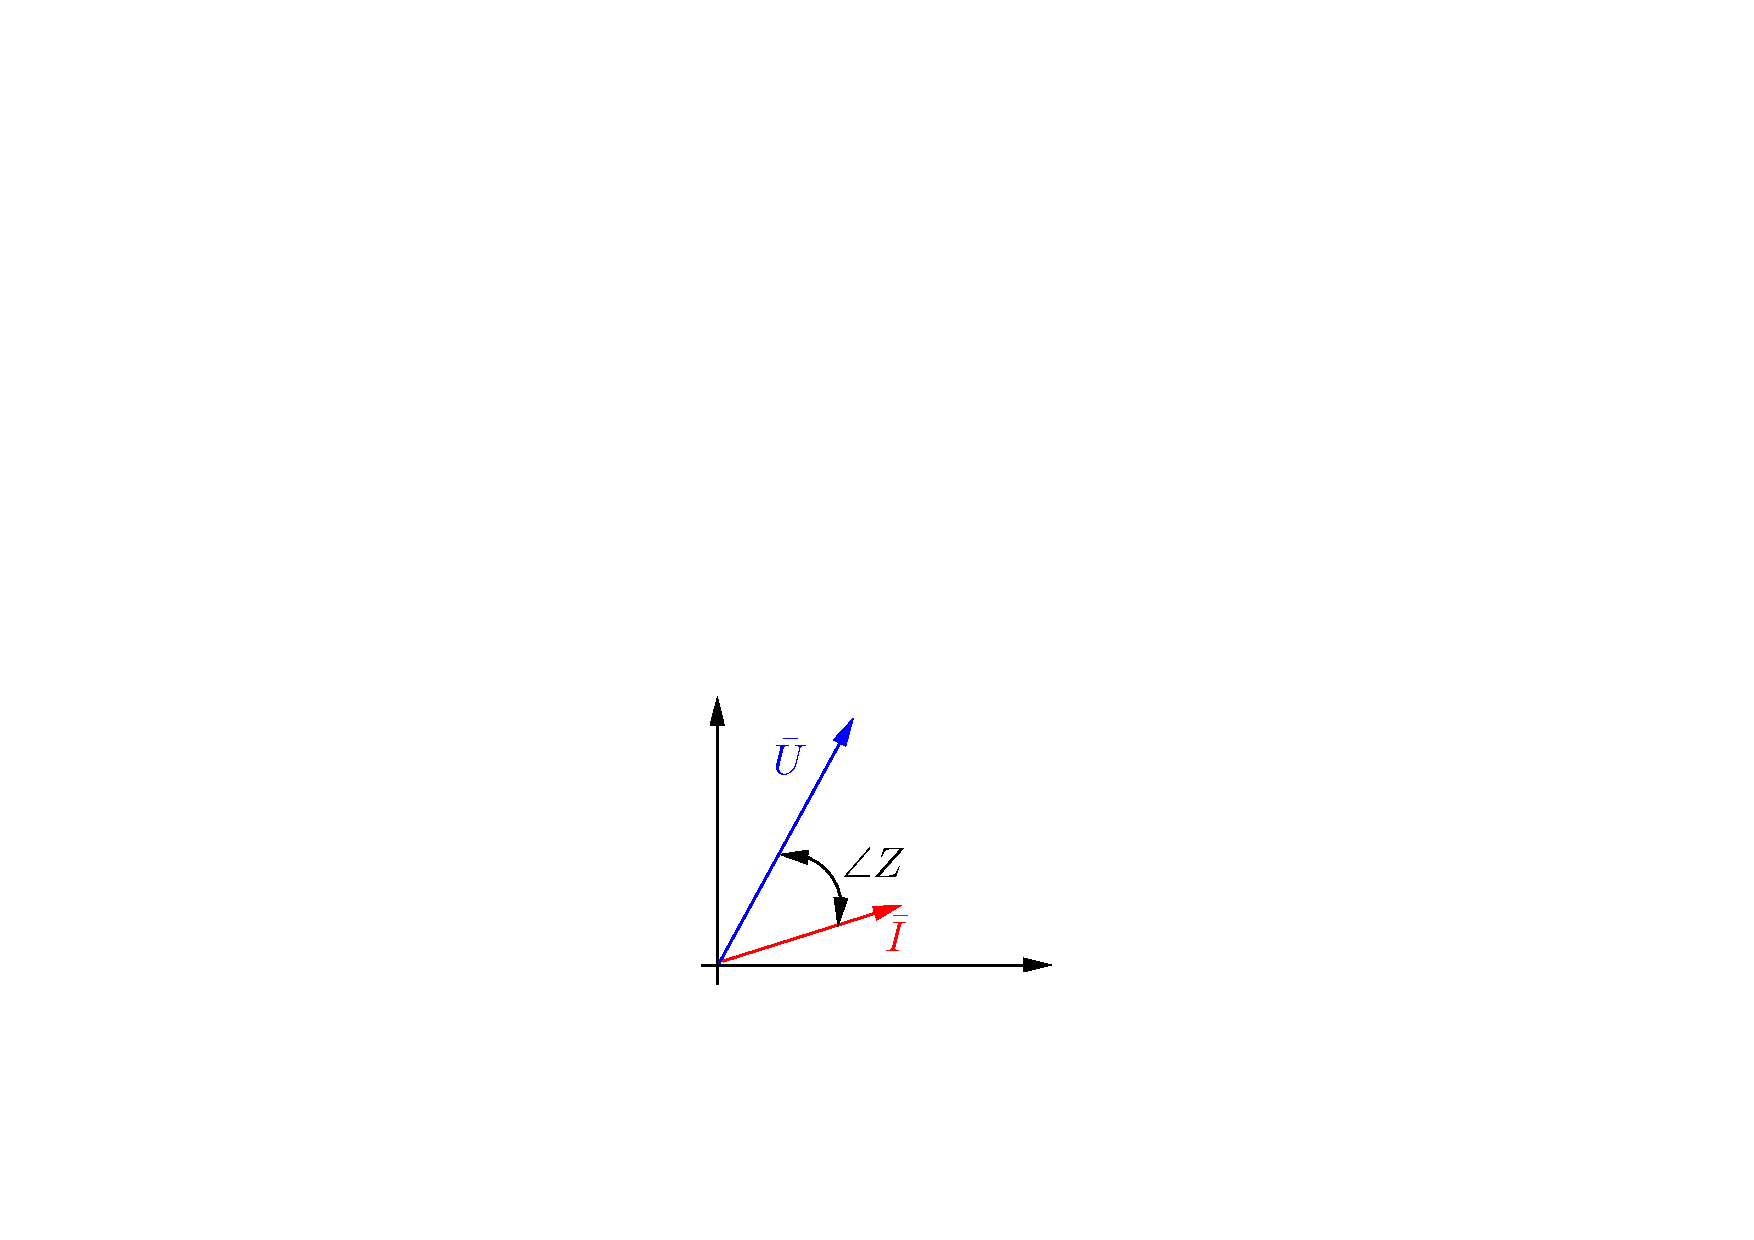
\includegraphics[width=\linewidth]{figs/Z_RLC}
    \end{center}
  \end{column}
\end{columns}

\begin{block}{Illustration}
Dans un simulateur : pour $R$ fixée, faire varier les valeurs de $L$ et $C$ et observer le déphasage.
Trouver une valeur pour $L \neq 0$ et pour $C \neq 0$ telle que le déphase est nul.
\end{block}

	
\end{frame}

%-------------------------------------------------------------------------------

\subsection{Formulation de l'approche fréquentielle}
\begin{frame}{Formulation de l'approche fréquentielle}
  \centering
	\includegraphics[width=0.8\linewidth]{"figs/approche frequentielle"}
\end{frame}

%-------------------------------------------------------------------------------

\subsection{Exerice}
\begin{frame}[allowframebreaks]{Exercice}
	\begin{columns}
  \begin{column}{0.45\textwidth}
    \begin{itemize}
      \item La source de courant délivre un courant $i(t)=\sqrt{2}\,8\cos 200\,000\,t$ A.
      \item Construire le schéma équivalent du circuit dans le domaine fréquentiel.
      \item Trouver les expressions temporelles de $u$, $i_1$, $i_2$ et $i_3$ en régime établi.
    \end{itemize}
  \end{column}
  \begin{column}{0.5\textwidth}
    \begin{center}
    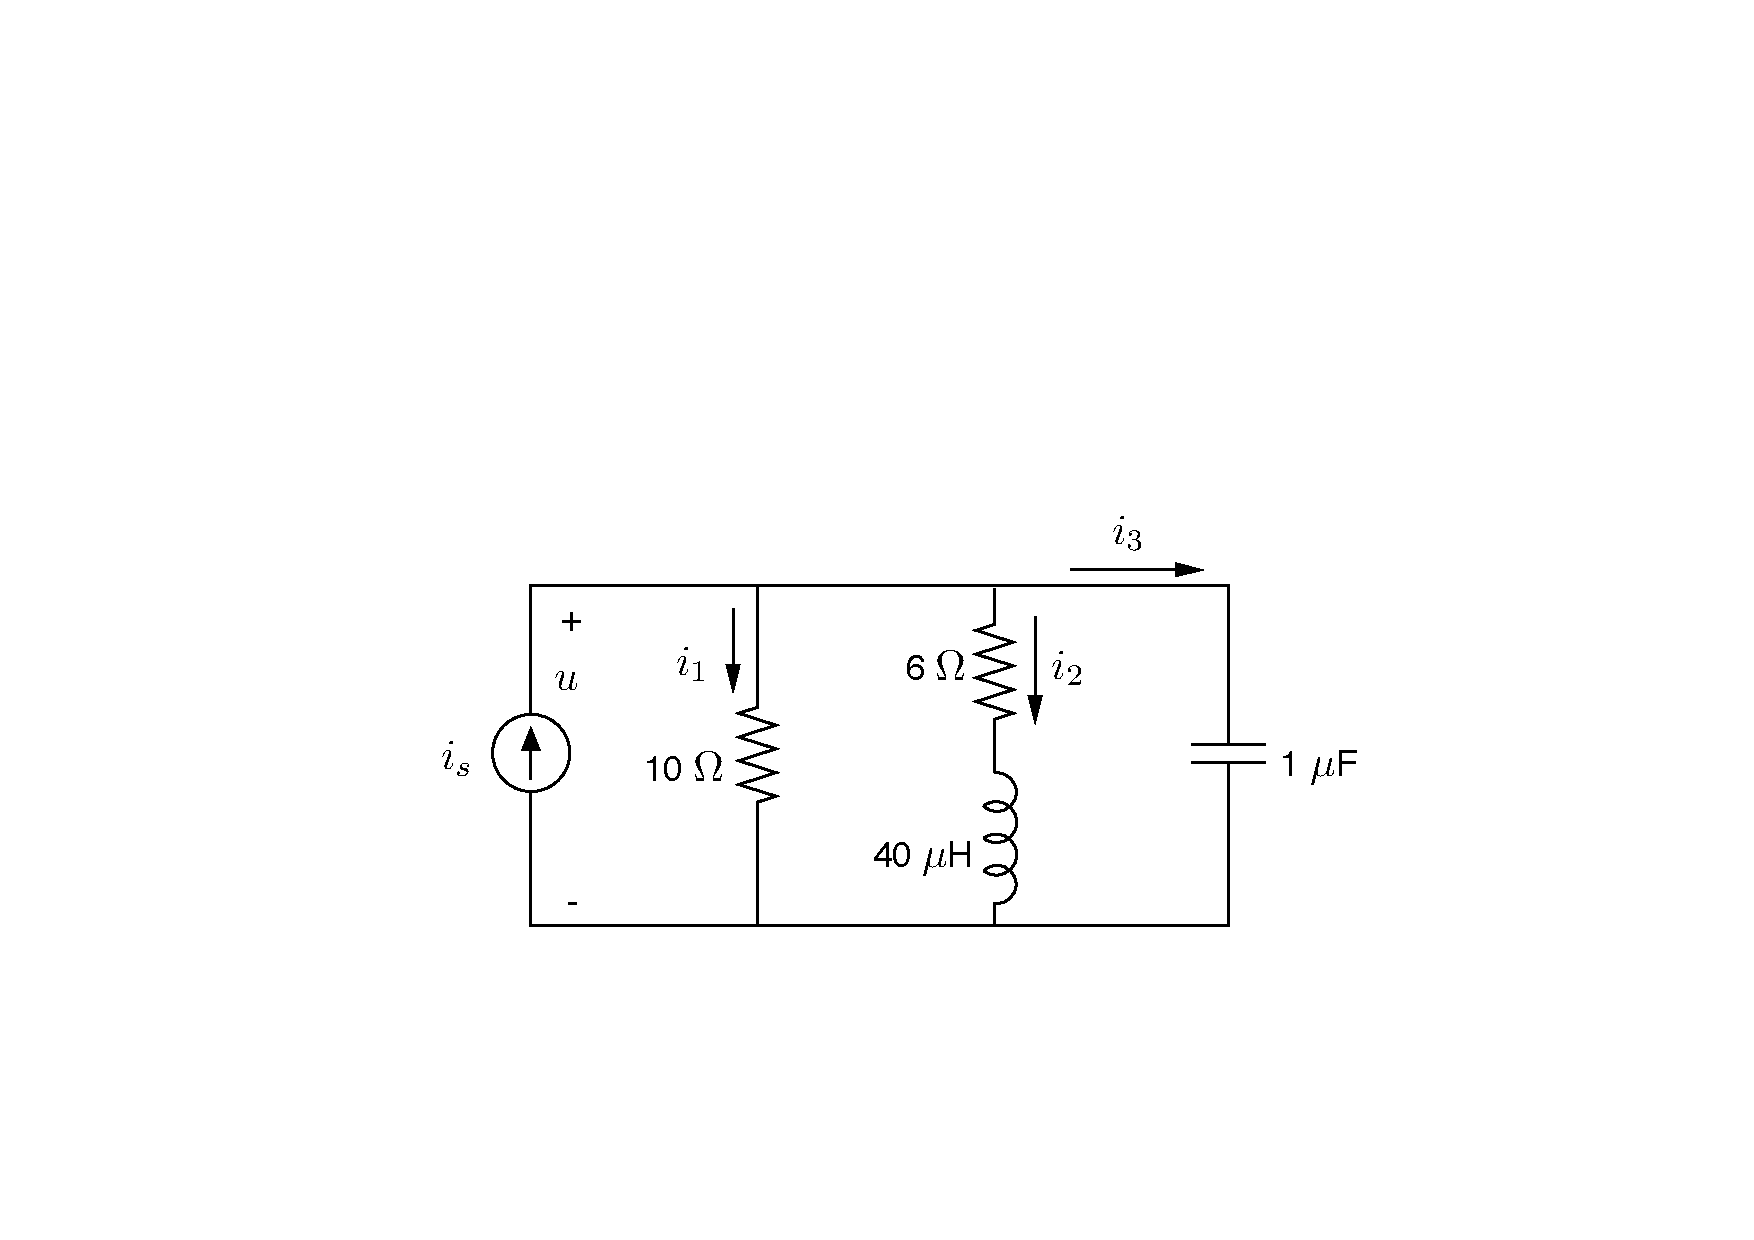
\includegraphics[width=\linewidth]{figs/exemple}
    \end{center}
  \end{column}
  \end{columns}
  
%-------------------------------------------------------------------------------

	
	\[\bar{I}=8\,\angle 0, \quad \omega L = 8\, \Omega\, , \quad
	\frac{-1}{\omega C}=-5\, \Omega\]
	\begin{center}
	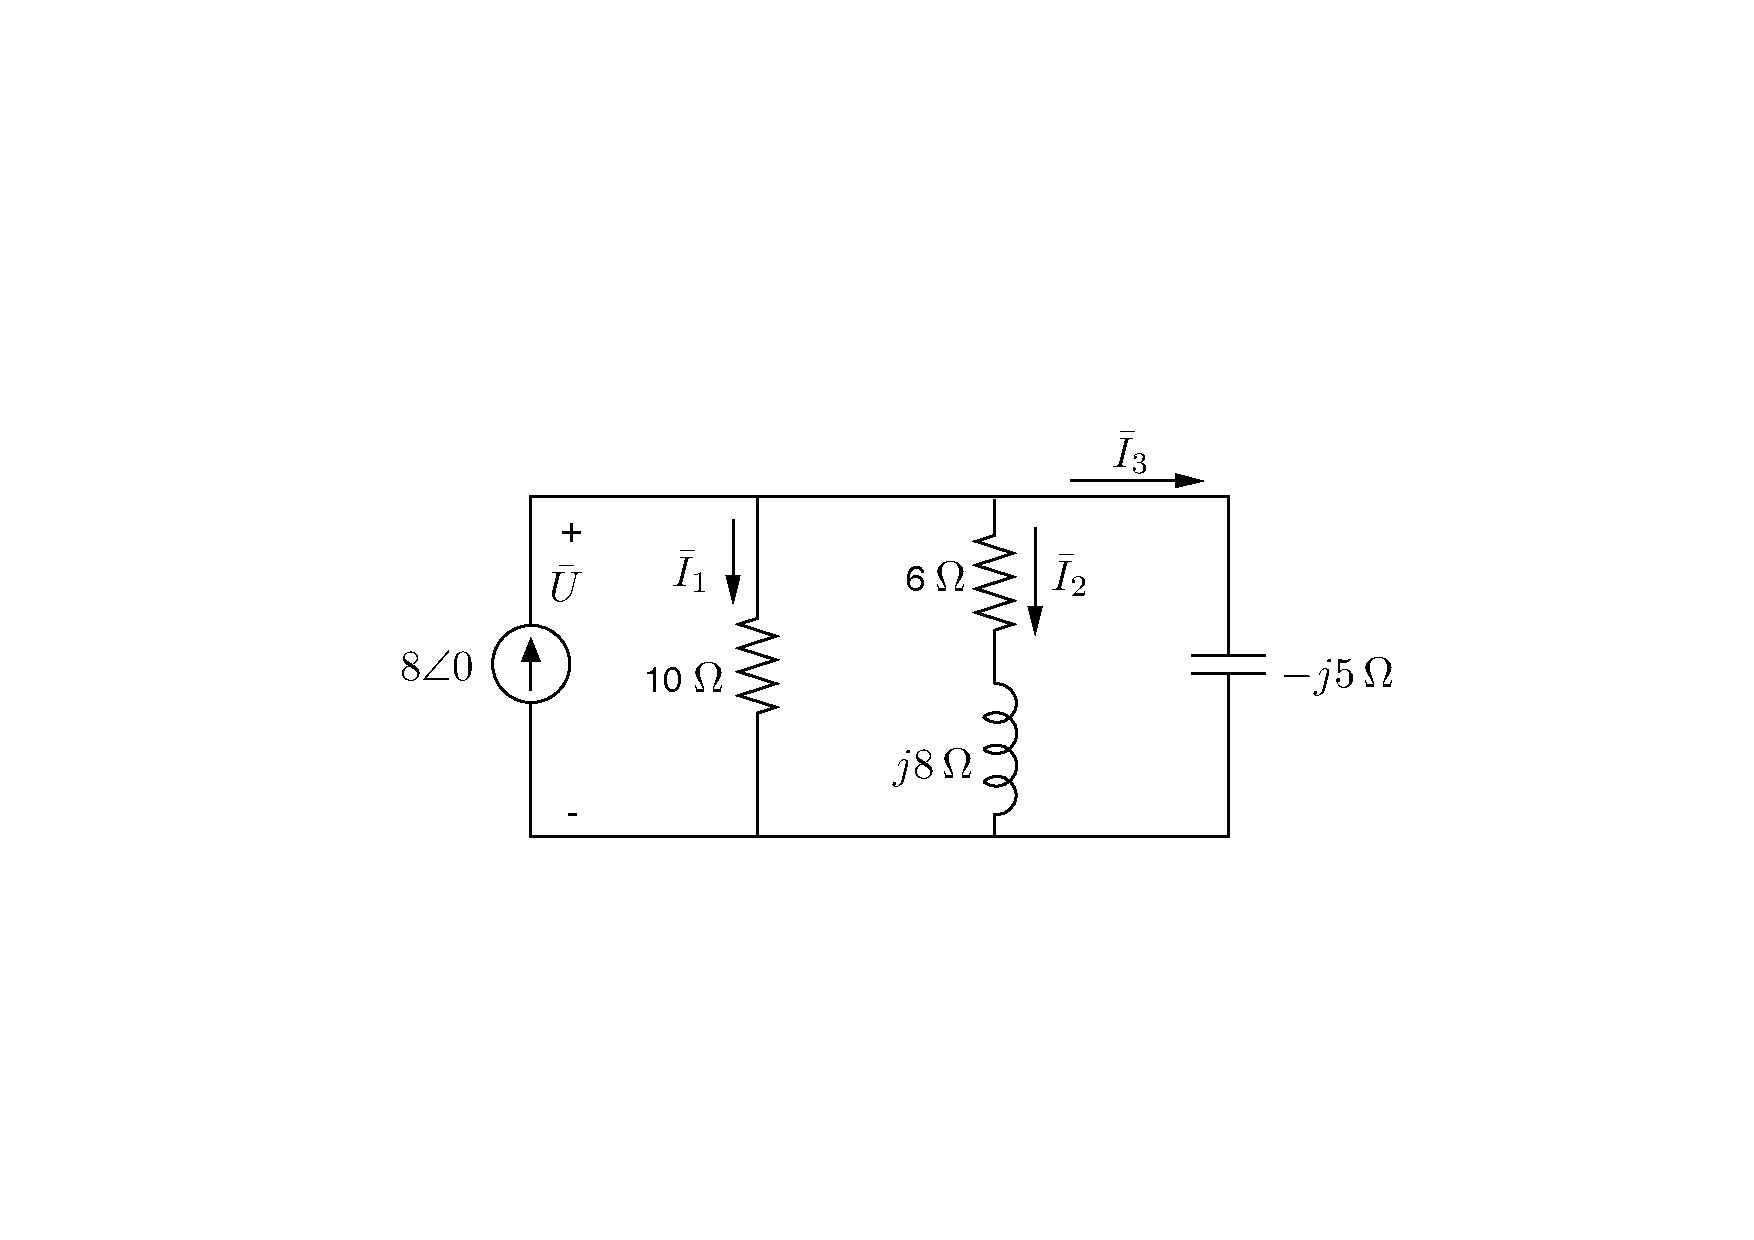
\includegraphics[width=0.7\linewidth]{figs/exemple_2}
	\end{center}


%-------------------------------------------------------------------------------

	\begin{columns}
		\begin{column}{0.5\linewidth}
	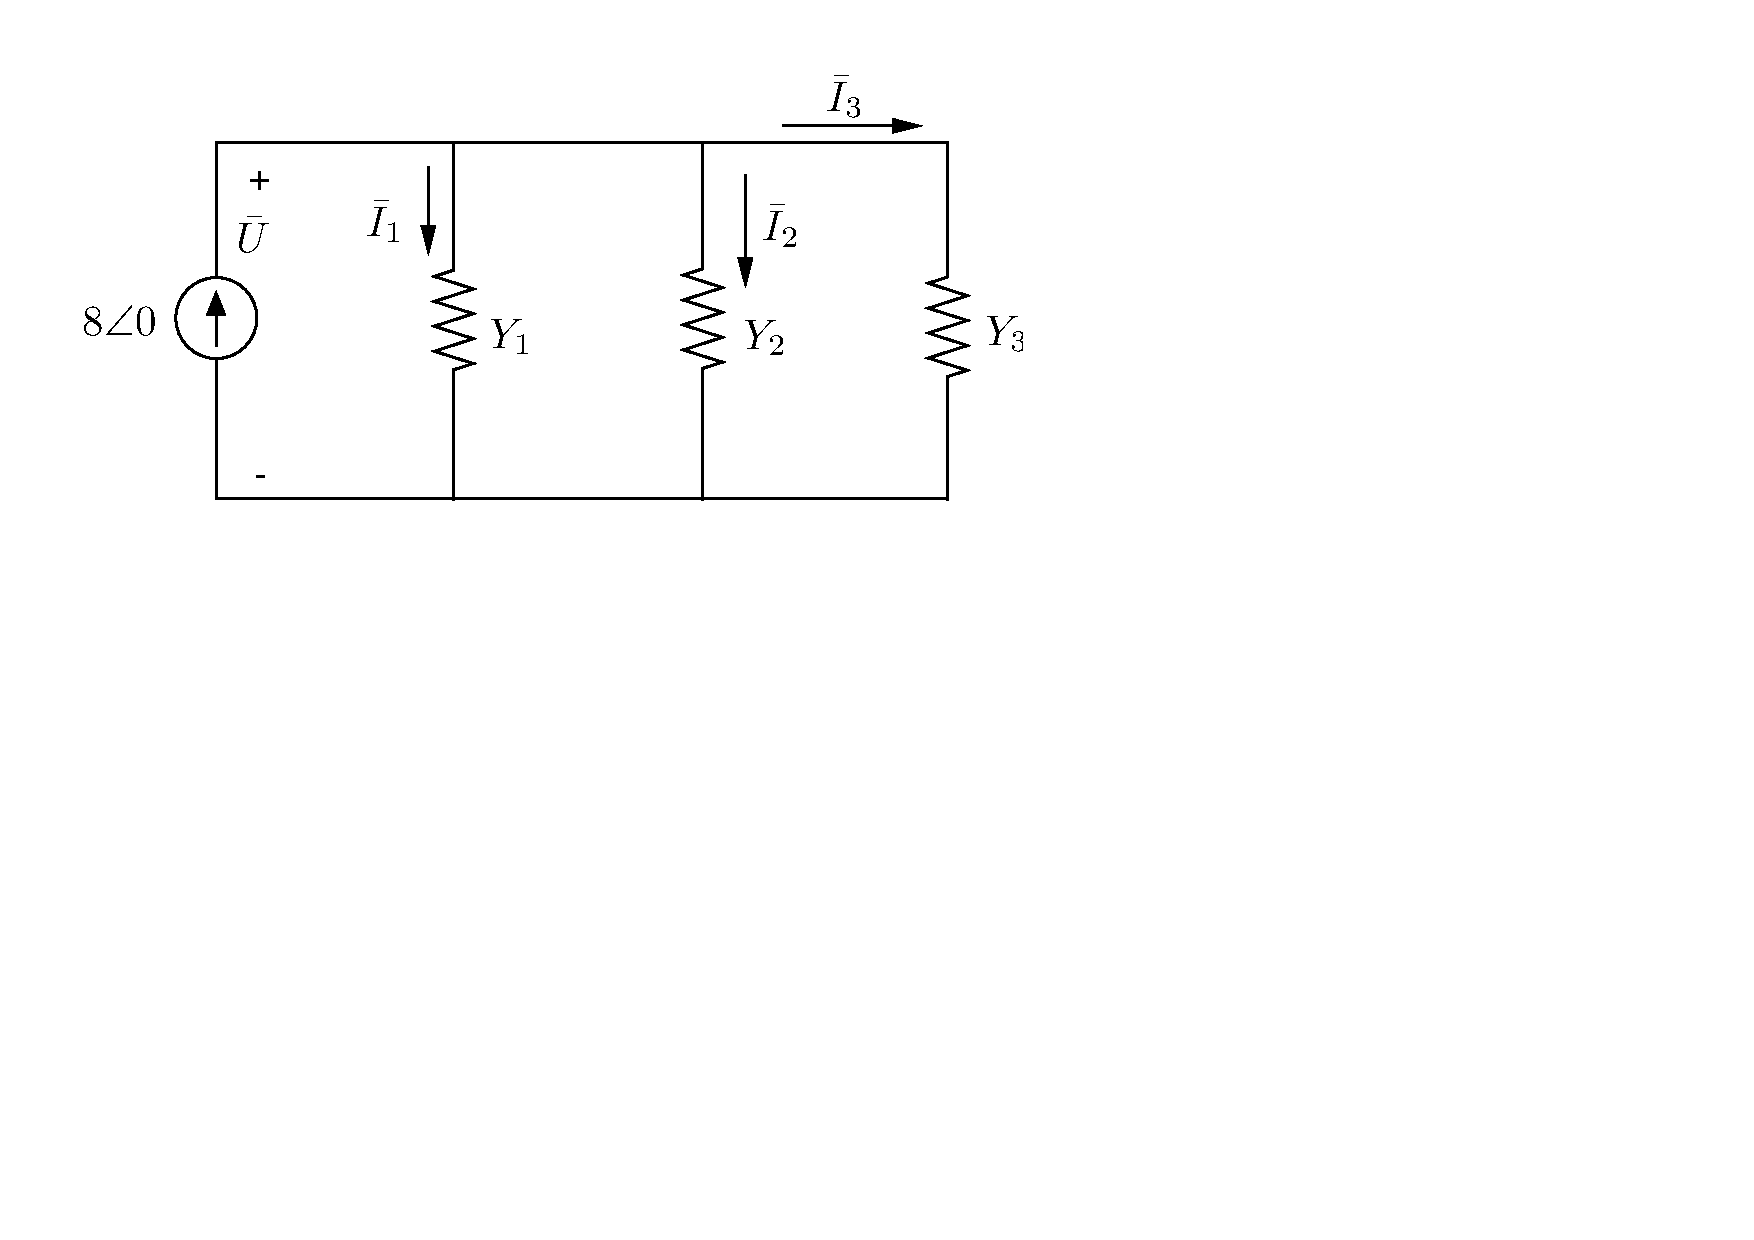
\includegraphics[width=0.9\linewidth]{figs/exemple_3}
		\end{column}
		\begin{column}{0.5\linewidth}
			 \begin{gather*}
				Y_1=\frac{1}{10}=0.1\, \text{S} \\
				Y_2=\frac{1}{6+j8}=0.06-j0.08\, \text{S}\\
				Y_3=j0.2\, \text{S}
				\end{gather*}
		\end{column}
	\end{columns}
	
		Admittance vue de la source :
		\[Y=Y_1+Y_2+Y_3=0.16+j0.12=0.2\angle 36.87^{\circ} \quad \rightarrow
		Z=\frac{1}{Y}=5\angle -36.87^{\circ}\]
		
		\begin{align*}
		\bar{U}&=Z\bar{I}=40\angle -36.87^{\circ}  &\rightarrow
		u(t)=\sqrt{2}\,40\cos(200\,000 t - 36.87^{\circ}) \text{V}\\
		\bar{I}_1&=Y_1\bar{U}=4\angle -36.87^{\circ}  &\rightarrow
		i_1(t)=\sqrt{2}\,4\cos(200\,000 t - 36.87^{\circ})\text{A} \\
		\bar{I}_2&=Y_2\bar{U}=4\angle -90^{\circ}  &\rightarrow
		i_2(t)=\sqrt{2}\,4\cos(200\,000 t - 90^{\circ})\text{A} \\
		\bar{I}_3&=Y_3\bar{U}=8\angle 53.13^{\circ}  &\rightarrow
		i_3(t)=\sqrt{2}\,8\cos(200\,000 t + 53.13^{\circ})\text{A}
		\end{align*}
\end{frame}